\documentclass[12pt,a4paper]{article}
\usepackage{fontspec,xunicode,xltxtra,amsmath,amsthm}
\XeTeXlinebreaklocale "zh"
\XeTeXlinebreakskip = 0pt plus 1pt minus 0.1pt
\newfontfamily\hei{黑体}
%\newfontfamily\song{SimSun}
\setmainfont{宋体}
%\usepackage[utf8]{inputenc}
\usepackage{tikz}
\usepackage{listings}
\lstset{frame=tb,
  language=SQL
}

\begin{document}

%========================================================================
\begin{center}
{
%\fontfamily{黑体}\selectfont
\hei
\vspace{80mm}
{\fontsize{32}{48}\selectfont 多媒体程序资源管理系统}

\vspace{30mm}
\textbf{\Huge{数据库设计文档}}\vspace{30mm}
}
\end{center}

\pagebreak

\noindent{\hei\Large 简介}\vspace{2mm}

本系统采用嵌入式关系型数据库SQLite存储图形程序需要维护的状态,%
用Haskell语言(选用的编译器是Glasgow Haskell Compiler)开发了一个自动维护OpenGL资源%
的程序。

\vspace{12mm}\noindent{\hei\Large 相关文档}\vspace{2mm}

[1] http://hackage.haskell.org/package/direct-sqlite

[2] http://www.sqlite.org/docs.html

[3] 《A First Course in Database Systems》\hfill 机械工业出版社

[4] 《Real World Haskell》\hfill 东南大学出版社

[5] The OpenGL\textregistered  Graphics System:A Specification (Version 3.1 - May 28, 2009)

[6] OpenGL 3.3 Reference Pages 
	
	\hspace{10mm} http://www.opengl.org/sdk/docs/man3/

[7] http://www.opengl.org/wiki/

\vspace{12mm}\noindent{\hei\Large 系统结构}\vspace{2mm}

本系统有三个进程,分别称为Player, Controller 和 Monitor.其中Player是实现真正资源管理的功能%
的演示程序。这三个进程通过读写内存中的同一数据库(Windows下只需下载一个RAM Disk的软件并在建立的%
RAM Disk中创建一个SQLite数据库文件即可,若是Linux下更是只需在/dev/shm下建立db文件)进行通信%
用户通过其它程序,或一系列的sql语句向位于内存中的数据库插入API无关的对绘图的描述,%
Player的一个线程按标记的时间顺序将API无关的描述连续地转化为对OpenGL的操作(状态绑定和绘图调用)%
的序列并存入数据库中,在转化时即进行缓冲区的创建和填充。%
Player的另一线程则按照真实的时间根据数据库的内容实际进行绘制。%
Controller具有GUI,接受用户的命令并向数据库中写入数据以控制Player显示哪一帧。%
Monitor定时(目前是10Hz)对Player中OpenGL资源的数量和总容量进行采样,并将结果存入另一个数据库中。%

\vspace{12mm}\noindent{\hei\Large E/R模型设计}\vspace{2mm}

\usetikzlibrary{er}
\tikzstyle{every weak entity} = [] 
\tikzstyle{weak entity} = [entity, double, double distance=2pt,every weak entity] 
\tikzstyle{ident relationship} = [relationship, double, double distance=2pt] 
\usetikzlibrary{arrows}

我们首先仅考虑单帧的情况,建立单帧模型之后再加入时间的概念,建立含时间的模型。
\vspace{10mm}
	\tikzstyle{every entity}=[draw=blue,fill=blue!10,thick]
	\tikzstyle{every relationship}=[fill=orange!10,draw=orange,thick]
	\tikzstyle{every attribute}=[draw=cyan,fill=cyan!10,thick]

\begin{center}
\begin{tikzpicture}[node distance=3cm,line width=0.5mm]
	\node[entity] (drawcall) at (0,0) {Draw Call} 
		child {node[attribute] at (-4,2){Primitive Type}}
		child {node[attribute] at (-5,0.5){Number of Instances}};
	\node[entity] (geometry) at (4,0) {Geometry};
	\node[weak entity] (program) at (0,3) {\parbox[t]{2cm}{\center Shader Binding}};
	\node[weak entity] (gsh) at (-5.5,2) {Geometry Shader};
	\node[weak entity] (vsh) at (0,6) {Vertex Shader};
	\node[weak entity] (fsh) at (-4.5,3.5) {Fragment Shader};
	\node[ident relationship] (has) at (-2.5,2){has}
		edge (program)
		edge [-)](gsh);
	\node[ident relationship] (has) at (0,4.5){has}
		edge (program)
		edge [-)](vsh);
	\node[ident relationship] (has) at (-2,3.5){has}
		edge (program)
		edge [-)](fsh);
	\node[relationship] (has) at (2,0){has}
		edge (drawcall)
		edge (geometry);
	\node[ident relationship] (has) at (0,1.5){has}
		edge (drawcall)
		edge (program);
	\node[weak entity] (scmat) at (-4,-3) {Shader Constant (Matrix)}
		child {node[attribute] at (-2,0){\underline{Name}}}
		child {node[attribute] {Elements(1..16)}};
	\node[weak entity] (scvec) at (3,-4.5) {Shader Constant (Vector)}
		child {node[attribute] at (-2,0){\underline{Name}}}
		child {node[attribute] {Elements(1..4)}};
	\node[ident relationship] (has) at (0,-1.5) {has} edge [-)] (drawcall) edge (scmat);
	\node[ident relationship] (has) at (1.5,-1.5) {has} edge [-)] (drawcall) edge (scvec);
	\node[entity] (gtype) at (4.5,5) {Geometry Type}
		child {node[attribute] at (-2.5,1.5) {\underline{Name}}};
	\node[relationship] (conforms) at (6,2.5) [text width=1.8cm,text centered	] {Conforms with} 
		edge (geometry) edge [-)] (gtype);	
	\node[relationship] (conforms) at (3,2.5) [text width=1.8cm,text centered	] {Conforms with}
		edge (vsh) edge [-)] (gtype);
	\node[weak entity] (va) at (5,8) {\parbox[t]{2cm}{\center Vertex \\ Attribute}}
		child {node[attribute] at (0,0) {\underline{Name}}}
		child {node[attribute] at (-3.5,1.5) {Type of Elements}}
		child {node[attribute] at (-3.5,3) {Dimension}}
		child {node[attribute] at (-1,3) {Volatility}};
	\node[ident relationship] (has) at (5,6.5) {has} edge (va) edge [-)] (gtype);
	\node[weak entity] (gd) at (6,-1.5) {Geometry Data}
		child {node[attribute] at (-1,0) {\underline{Index}}}
		child {node[attribute] {Value}};
	\node[ident relationship] at (8,3) {Cw}
		edge(va) edge[-)](gd);
	\node[ident relationship] (has) at (6,0) {has} edge [-)] (geometry) edge(gd);
	\node[weak entity] (text) at (-5,6) {Text Resource}
		child {node[attribute] at (-1.5,3) {Text}};
	\node[ident relationship] (is) at (-4.5,4.7) {is} edge[-)](text) edge(fsh);
	\node[ident relationship] (is) at (-7,3.5) {is} edge[-)](text) edge(gsh);
	\node[ident relationship] (is) at (-2.5,6) {is} edge[-)](text) edge(vsh);
	\node[entity] (res) at (-3.5,9) {Resource}
		child {node[attribute] at (-2.5,1.5) {\underline{Name}}}
		child {node[attribute] at (-3.5,3) {\underline{Type}}};
	\node[ident relationship] (is) at (-4,7.5) {is} edge(text) edge[-)](res);
	\node[weak entity] (file) at (-2,11) {Resource From File}
		child {node[attribute] at (4,1.5) {Filename}};
	\node[ident relationship] (is) at (-1.5,9.5) {is}
		edge [-)](res)
		edge (file);
\end{tikzpicture}
图2-1
\end{center}

\newpage
对于OpenGL的状态则有:

\begin{center}
\begin{tikzpicture}[node distance=3cm,line width=0.5mm]
	\node[entity] (glo) {GL Object} 
		child {node[attribute] at (-1,0) {\underline{ID}}}
		child {node[attribute] {\underline{Object Type}}};
	\node[weak entity] (glb) at (5,0) {GL Buffer Object}
		child {node[attribute] {Buffer Type}};
	\node[ident relationship] (is) at (2,0) {is}
		edge [-)](glo) edge (glb);
	\node[weak entity] (gls) at (-5,0) {GL Shader Object}
		child {node[attribute] {Shader Type}};
	\node[ident relationship] (is) at (-2,0) {is}
		edge [-)](glo) edge (gls);
	\node[weak entity] (glp) at (-5,7.5) {GL Program};
	\node[ident relationship] at (-0.5,6.5) {is}
		edge [-)](glo) edge (glp);
	\node[relationship] (vs) at (-6.5,3.5) 
		{\parbox[t]{2cm}{\center Use as \\ Vertex \\ Shader}}
		edge [-)](gls) edge (glp);
	\node[relationship] (fs) at (-2.5,3.5) 
		{\parbox[t]{2cm}{\center Use as \\ Fragment \\ Shader}}
		edge [-)](gls) edge (glp);
	\node[relationship] (gs) at (2,3.5)
		{\parbox[t]{2cm}{\center Use as \\ Geometry \\ Shader}}
		edge [-)](gls) edge (glp);
	\node[weak entity] (gln) at (5,2) {Named Object};
	\node[ident relationship] at (3,1.5) {is}
		edge [-)](glo) edge (gln);
	\node[weak entity] (glv) at (-2,-3) {GL Vertex Array Object};
	\node[ident relationship] at (-2.7,-1) {is}
		edge [-)](glo) edge (glv);
\end{tikzpicture}
图2-2
\end{center}

\newpage
接下来从图2-1出发,给随时间变化的实体/关系加上时间。略去没有变化的部分。
\begin{center}
\begin{tikzpicture}[node distance=3cm,line width=0.5mm]
	\node[entity] (drawcall) at (0,0) {Draw Call} 
		child {node[attribute] at (-3,2){Primitive Type}}
		child {node[attribute] at (-5,0.5){\parbox[t]{2cm}{Number of \\ Instances}}}
		child {node[attribute] at (-3.5,0){\underline{Time}}};
	\node[entity] (geometry) at (4,0) {Geometry};
	\node[weak entity] (program) at (0,3) {Shader Binding};
	\node[ident relationship] (has) at (0,1.5){has}
		edge (drawcall)
		edge (program)
		child {node[attribute] at (-1.5,1.5) {Time}};
	\node[relationship] (has) at (2,0){has}
		edge (drawcall)
		edge (geometry)
		child {node[attribute] at (0,3) {Time}};
	\node[weak entity] (scmat) at (-4,-4) {Shader Constant (Matrix)}
		child {node[attribute] at (-1,0){\underline{Name}}}
		child {node[attribute] at (1,0){Elements(1..16)}}
		child {node[attribute] at (-3.5,3){\underline{Time}}};
	\node[weak entity] (scvec) at (3,-5) {Shader Constant (Vector)}
		child {node[attribute] at (-2,0){\underline{Name}}}
		child {node[attribute] {Elements(1..4)}}
		child {node[attribute] at (-3.5,3) {\underline{Time}}};
	\node[ident relationship] (has) at (0,-1.5) {has} edge [-)](drawcall) edge (scmat);
	\node[ident relationship] (has) at (1.5,-1.5) {has} edge [-)](drawcall) edge (scvec);
	\node[weak entity] (gd) at (6,-1.5) {Geometry Data}
		child {node[attribute] at (-1,0) {\underline{Index}}}
		child {node[attribute] {Value}}
		child {node[attribute] at (-4,1.5){\underline{Time}}};
	\node[ident relationship] (has) at (6,0) {has} edge [-)](geometry) edge(gd);
	\node[weak entity] (va) at (5,2) {\parbox[t]{2cm}{\center Vertex \\ Attribute}};
	\node[ident relationship] (cw) at (7,0.5) {Cw} edge (gd) edge [-)](va);
\end{tikzpicture}

\vspace{10mm}
图2-3
\end{center}

\vspace{2cm}
由于时间上的冗余性(对于某一实体,在t帧取值和在(t+1)帧取值不同的概率很小),因此将%
Time属性改为Time-Start, 表示一段时间内的取值。对于Draw Call, 因为需要表达"在某些时刻%
不存在",因此显式地加上Time-End. 然而在Draw Call本身不存在的时刻其相关属性有定义也不会%
有坏处,反而能减少数据量。因此Draw Call除时间外的相关属性全部作为实体处理,且只具有Time-Start,而Time-End隐含%
在下一个Time-Start中。此外,为了减少数据量也给部分实体加上名字作为主键。此处考虑到现代显卡的%
工作方式,不适合处理少量高频变化的顶点数据(如果有这种情况应该转化为shader的常数处理),%
而应当一次上传一批数据,因此加入Geometry Data Relational这个实体。
同样省略掉和单帧情形相比无变化的部分。由于各属性的时间可以独立变化因此一些完整性条件也消失了。

\begin{center}
\begin{tikzpicture}[node distance=3cm,line width=0.5mm]
	\node[entity] (drawcall) at (-2,0) {Draw Call} 
		child {node[attribute] at (-2,0){\underline{Time-Start}}}
		child {node[attribute] at (-4,1.5){Time-End}}
		child {node[attribute] at (-4,3){\underline{Name}}};
	\node[weak entity] (dcp) at (-1,3) {Draw Call Prop}
		child {node[attribute] at (-1,3) {\underline{Time-Start}}}
		child {node[attribute] at (-5,1.5){Primitive Type}};
		%child {node[attribute] at (-5,0.5){Number of Instances}};
	\node[weak entity] (program) at (4,-8) {Shader Binding}
		child {node[attribute] {\underline{Time-Start}}};
	\node[ident relationship] (has) at (0.5,-6.5){has}
		edge (drawcall)
		edge (program);
	\node[ident relationship] (has) at (-0.5,1.5) {has}
		edge (drawcall) edge (dcp);
	\node[entity] (geometry) at (2.5,0) {Geometry}
		child {node[attribute] at (-2,1.5){\underline{Name}}};
	\node[weak entity] (gd) at (5.5,0) {Geometry Data}
		child {node[attribute] at (-1.5,3) {Index}}
		child {node[attribute] at (-1,3){Value}};
	\node[weak entity] (gdr) at (3,-3) {\parbox[t]{3cm}{\center Geometry Data \\ Relational}}
		child {node[attribute] at (0.5,0) {Number of Elements}}
		child {node[attribute] at (0,3) {\underline{Time-Start}}};
	\node[weak entity] (va) at (4.5,-6) {\parbox[t]{2cm}{\center Vertex \\ Attribute}};
	\node[ident relationship] (cw) at (6.5,-4.5) {Cw} edge (gdr) edge [-)](va);
	\node[ident relationship] (has) at (6,-2) {has} edge [-)](gdr) edge(gd);
	\node[ident relationship] (has) at (0.5,-1.5) {has}
		edge (gdr) edge [-)](geometry);
	\node[relationship] (has) at (1.5,1.5){has}
		edge (dcp)
		edge [-)] (geometry);
	\node[weak entity] (scmat) at (-4,-4) {Shader Constant (Matrix)}
		child {node[attribute] at (-2,0){\underline{Name}}}
		child {node[attribute] {Elements(1..16)}}
		child {node[attribute] at (-4,3){\underline{Time-Start}}};
	\node[weak entity] (scvec) at (-2,-8) {Shader Constant (Vector)}
		child {node[attribute] at (-2,0){\underline{Name}}}
		child {node[attribute] {Elements(1..4)}}
		child {node[attribute] at (-2.5,3) {\underline{Time-Start}}};
	\node[ident relationship] (has) at (-2.5,-1.5) {has} edge (drawcall) edge (scmat);
	\node[ident relationship] (has) at (-0.5,-6) {has} edge (drawcall) edge (scvec);
	\node[weak entity] (inst) at (0.5,6) {Instancing}
		child {node[attribute] at (-4.5,1.5) {Number of Instances}}
		child {node[attribute] at (-3.5,3) {\underline{Time-Start}}};
	\node[ident relationship] (has) at (0,4.5) {has} edge [-)] (dcp) edge [->](inst);
\end{tikzpicture}

\vspace{10mm}
图2-4
\end{center}

\newpage
用户输入的数据遵循图2-4所示的模型,和API是无关的,并且也不需要考虑如何维护显示用的各种资源。%
接下来是将该API无关模型的数据映射到OpenGL的各种Objects,向缓冲区中装入数据。%
为了控制图的大小,该部分与图2-4中及图2-2中的模型的部分连接(即原图中的部分Entity sets的key)%
仅作为该模型中的Entity set%
的Attributes画出,而不画出原图中出现过的Entity sets.%
原图中出现过的Entity sets在下图中画出时不画出其Attributes.

\vspace {10mm}
\noindent 第一部分:
\begin{center}
\begin{tikzpicture}[node distance=5cm,line width=0.5mm]
	\node[weak entity] (sdcp) at (-4,5){\parbox[t]{3cm}{\center{Synchronized \\ Draw Call Prop}}}
		child {node[attribute] {\underline{Time-Start}}};
	\node[weak entity] (ssb) at (4,5) {\parbox[t]{3cm}{\center{Synchronized \\ Shader Binding}}}
		child {node[attribute] {\underline{Time-Start}}};
	\node[weak entity] (sscm) at (-4,0) {\parbox[t]{3cm}{\center{Synchronized \\ Shader Constant \\ (Matrix)}}}
		child {node[attribute] at (5.5,1){\underline{Time-Start}}}
		child {node[attribute] at (0,3.5) {Elements(1..16)}}
		child {node[attribute] at (0,-1.5) {GL Uniform Location}};
	\node[weak entity] (sscv) at (4,0) {\parbox[t]{3cm}{\center{Synchronized \\ Shader Constant \\ (Vector)}}}
		child {node[attribute] at (0,-2.5) {GL Uniform Location}}
		child {node[attribute] at (0,3.5) {Elements(1..4)}}
		child {node[attribute] at (-5.5,-0.5){\underline{Time-Start}}};
	\node[entity] (dc) at (0,3) {Draw Call};
	\node[entity] (inst) at (-5,8) {Instancing};
	\node[entity] (glv) at (-1,8) {GL Vertex Array Object};
	\node[entity] (glp) at (5,8) {GL Program};
	\node[relationship] at (-5,6.5) {has} edge [->] (inst) edge(sdcp);
	\node[relationship] at (-1,6.5) {has} edge [-)] (glv) edge (sdcp);
	\node[relationship] at (5,6.5) {has} edge [-)] (glp) edge (ssb);
	\node[ident relationship] at (1,5) {is for} edge [-)] (dc) edge (ssb);
	\node[ident relationship] at (-1,5) {is for} edge [-)] (dc) edge (sdcp);
	\node[ident relationship] at (1,1) {is for} edge [-)] (dc) edge (sscv);
	\node[ident relationship] at (-1,1) {is for} edge [-)] (dc) edge (sscm);
\end{tikzpicture}

\vspace{10mm}
图2-5
\end{center}

\newpage
\noindent 第二部分:
\begin{center}
\begin{tikzpicture}[node distance=5cm,line width=0.5mm]
	\node[weak entity] (gi) at (0.5,-1) {Geometry Implementation}
		child {node[attribute] at (2,3){\underline{Time-Start of Implementation}}};
	\node[weak entity] (ag) at (0,3.5) {Vertex Attribute Group}
		child {node[attribute] at (2.5,0){\underline{Attribute Group ID}}}
		child {node[attribute] at (-3,3){Stride}};
	\node[weak entity] (ab) at (0,7) {\parbox[t]{3cm}{\center Automatically \\ Generated \\ Buffer}};
	\node[entity] (g) at (5,-3) {Geometry};
	\node[entity] (glv) at (1,-3) {GL Vertex Array Object};
	\node[relationship] at (-2.5,-2.5) {has} edge (gi) edge [-)] (glv);
	\node[ident relationship] at (5,-1) {is for} edge (gi) edge [-)] (g);
	\node[ident relationship] at (-3,0.5) {has} edge [-)] (gi) edge (ag);
	\node[entity] (va) at (4.5,5) {\parbox[t]{2cm}{\center Vertex \\ Attribute}};
	\node[relationship] at (3.5,3.5) {has}
		edge (va) edge (ag)
		child {node[attribute] at (1.5,1) {Offset}};
	\node[entity] (glb) at (0,10) {GL Buffer Object}
		child {node[attribute] at (2,3) {Reference Count}};
	\node[ident relationship] at (0,5) {has} edge (ab) edge [-)] (ag);
	\node[relationship] at (-2,8.5) {is} edge [-)] (ab) edge (glb);
	\node[relationship] at (3,7) {binds} edge [-)] (ag) edge (glb)
		child {node[attribute] at (1.5,3) {Time-Start}};
\end{tikzpicture}

\vspace{10mm}
图2-6
\end{center}

\newpage

\vspace{12mm}\noindent{\hei\Large Schema设计}\vspace{2mm}

所有主键均以UNIQUE处理。

\noindent (1) 图2-1,图2-3,图2-4中的E/R模型:
\begin{lstlisting}
draw_calls(name,time_start,time_end,
	UNIQUE (name,time_start));
draw_call_prop(dc_name,time_start,prim_type,geometry_name,
	instancing,UNIQUE (dc_name,time_start));
shader_binding(dc_name,time_start,vertex_shader_name,
	geometry_shader_name,fragment_shader_name,
	UNIQUE (time_start,dc_name));
instancing(dc_name,time_start,instances,
	UNIQUE (time_start,dc_name));
shader_constants_m44(dc_name,time_start,var_name ,
	m11 , m12 , m13 , m14 , 
	m21 , m22 , m23 , m24 , 
	m31 , m32 , m33 , m34 ,
	m41 , m42 , m43 , m44 ,
	UNIQUE (time_start, dc_name, var_name) 
);
shader_constants_v4(dc_name,time_start,var_name,
	v1,v2,v3,v4,UNIQUE (time_start, dcname, var_name));
geometry_type_attrib_def(geometry_type_name,attrib_name,
	scalar_type,vec_dim,volatility,
	UNIQUE (geometry_type_name,attrib_name));
geometry_typing(geometry_name,geometry_type_name,
	UNIQUE (geometry_name));
vertex_shader_typing(vertex_shader_name,
	geometry_type_name,UNIQUE (vertex_shader_name));
geometry_data_relational(geometry_name,attrib_name,
	time_start,num_elements,
	UNIQUE(geometry_name,attrib_name,time_start));
geometry_data(geometry_name,attrib_name,time_start,i,value,
	UNIQUE(geometry_name,attrib_name,time_start,i));
text_res(type,name,data,UNIQUE(type,name));
file_res(type,name,filename,UNIQUE(type,name));
\end{lstlisting}

\newpage
\noindent (2) 图2-2中的E/R模型:
\begin{lstlisting}
gl_objects(type,gl_id,UNIQUE (type,gl_id));
gl_object_naming(type,gl_id,name,
	UNIQUE (type,gl_id),UNIQUE (type,name));
gl_buffer_objects(gl_id,type,UNIQUE (gl_id));
gl_shaders(gl_id,type,UNIQUE (gl_id));
gl_programs(vs_id,gs_id,fs_id,program_id,
	UNIQUE (vs_id, gs_id, fs_id),UNIQUE (program_id));
\end{lstlisting}

\vspace{10mm}
\noindent (3) 图2-5,图2-6中的E/R模型:
\begin{lstlisting}
gl_sync_geometry_impl(geometry_name,impl_time_start,
	gl_vao_id,UNIQUE(geometry_name,impl_time_start));
gl_sync_geometry_impl_attrib_groups(geometry_name,
	impl_time_start,attrib_group_id,stride,
	UNIQUE(geometry_name,impl_time_start,attrib_group_id));
gl_sync_geometry_length(gl_vao_id,time_start,length,
	UNIQUE(gl_vao_id,time_start));
gl_sync_geometry_attrib_in_group(geometry_name,
	impl_time_start,attrib_name,attrib_group_id,offset,
	UNIQUE(geometry_name,impl_time_start,attrib_name),
	UNIQUE(geometry_name,impl_time_start,
	attrib_group_id,offset));
gl_sync_geometry_attrib_group_has_auto_buffers(
	geometry_name,impl_time_start,attrib_group_id,
	gl_buffer_id,ref_count,
	UNIQUE(geometry_name,impl_time_start,
	attrib_group_id,gl_buffer_id));
gl_sync_gl_vao_buffer_binding(gl_vao_id,time_start,
	attrib_group_id,gl_buffer_id,
	UNIQUE(time_start,gl_vao_id,attrib_group_id)
	UNIQUE(time_start,gl_vao_id,gl_buffer_id));
gl_sync_draw_call_prop(dc_name,time_start,prim_type,
	gl_vao_id,instancing,UNIQUE (dc_name,time_start));
gl_sync_shader_binding(dc_name,time_start,program_id,
	UNIQUE(time_start,dc_name));
gl_sync_shader_constants_m44(dc_name,time_start,
	uniform_location,
	m11, m12, m13, m14, 
	m21, m22, m23, m24, 
	m31, m32, m33, m34,
	m41, m42, m43, m44,
	UNIQUE(time_start,dc_name,uniform_location));
gl_sync_shader_constants_v4(dc_name,time_start,
	uniform_location,v1,v2,v3,v4,
	UNIQUE (time_start,dc_name,uniform_location));
\end{lstlisting}

\vspace {10mm}
\noindent (4) 一些临时存放查询结果的表,不遵循E/R模型。
\begin{lstlisting}
gl_sync_gl_vao_buffer_has_vas(
	gl_vao_id,
	time_start,
	attrib_group_id,
	attrib_name,
	gl_va_id,
	gl_vec_dim,
	gl_type,
	gl_normalized,
	gl_stride,
	gl_pointer
);
cur_frame_draw_calls(dc_name);
cur_frame_gl_dcs(
	dc_name,
	prim_type,
	gl_vao_id,
	instancing,
	program_id,
	prim_first,
	prim_count
);
gl_sync_reqs_named(name,time_start,type);
\end{lstlisting}

\newpage
\noindent (5) 用于记录和控制帧号的表,只有一条记录,做成表是为了放在SQLite中%
便于进程间共享。
\begin{lstlisting}
CREATE TABLE playback_control(
	sync_start,sync_end,force_to_play,just_played);
\end{lstlisting}


\vspace{12mm}\noindent{\hei\Large 对API的改进}\vspace{2mm}

由于Haskell本身并不算在工业界广泛运用的语言,因此其OpenGL和SQLite的API均不太成熟,%
尤其是文档不详细。一些与C API相比抽象层次更高的API反而因无法参考C API的文档而难以使用。%
因此我选择了较为接近OpenGL和SQLite原本的C语言API的Haskell API,%
并作出了少量修改。OpenGL的部分略去不表,(修改后的代码在Graphics/下)。SQLite的%
Haskell API选用的是 direct-sqlite [1],修改后的代码在Database/下,加上主目录内的SQLUtil.hs。%
主要增加了这些函数:

\vspace{5mm}
\begin{lstlisting}
runStrB::Database->String->[SQLData]->IO [[SQLData]]
runStr db s = runStrB db s []
\end{lstlisting}

将字符串作为一条SQL语句执行,并返回结果。第二个函数用于没有binded variable的情况。

\vspace{5mm}
\begin{lstlisting}
runScript::Database->String->[SQLData]->IO [[[SQLData]]]
\end{lstlisting}

将字符串作为一条或多条SQL语句执行,并返回结果。这样可以将一长串SQL命令放在外部文件中一次读取并执行

\vspace{5mm}
这几个函数使得进行一次SQL调用往往只需要一行程序,使程序更精简。

\newpage
\vspace{12mm}\noindent{\hei\Large 图形界面}\vspace{2mm}

Player的图形界面就是一个GLUT窗口。	

\vspace{5mm}\noindent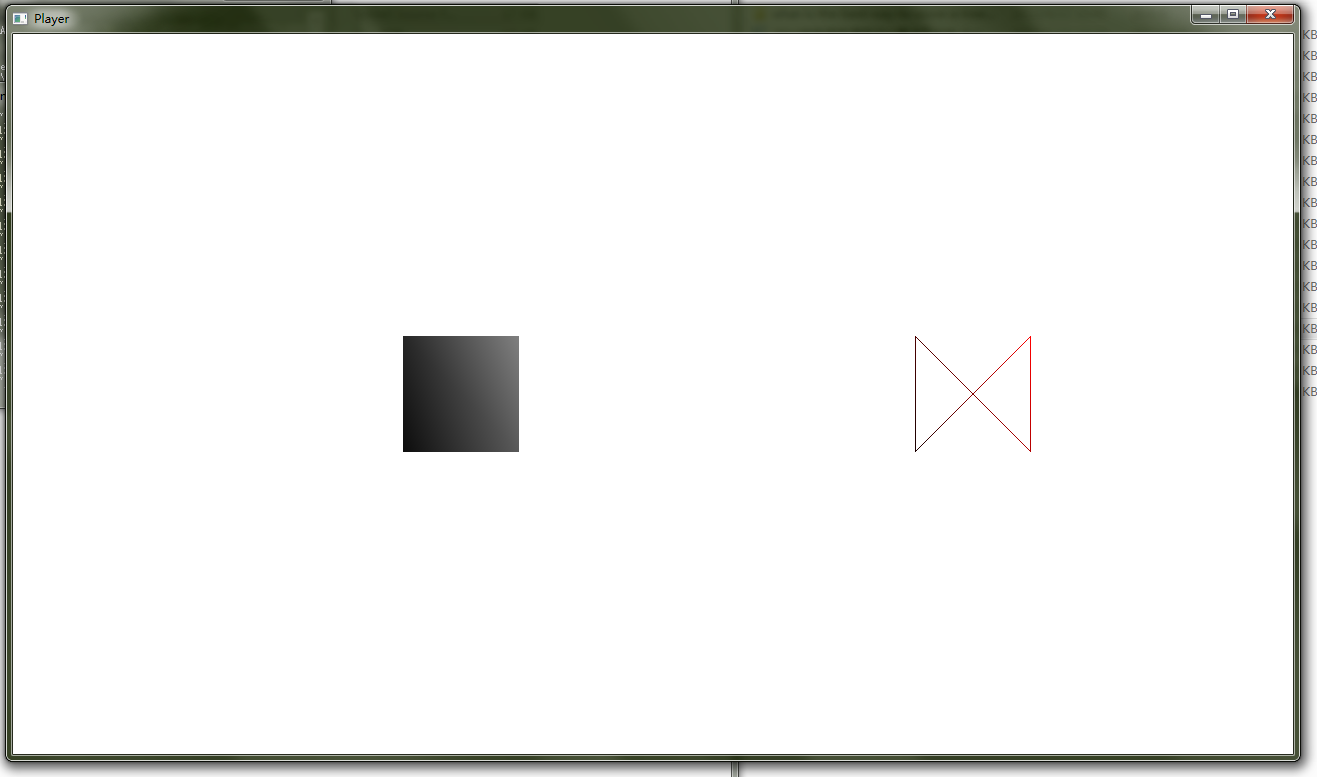
\includegraphics[width=\textwidth]{p0.png}\vspace{10mm}

Monitor没有图形界面。

\vspace{20mm}
Controller的图形界面采用Gtk2hs(也就是GTK的Haskell绑定)编写。主界面为

\vspace{5mm}\begin{center}
\includegraphics[width=60mm]{p1.png}\end{center}\vspace{10mm}
其中Play和Pause两个按钮控制通过向playback\_control这个表中写数据来控制Player是否按真实时间渲染帧。%
无论Player渲染到哪一帧,Player总是尽可能地按时间顺序载入各种资源。点击Load Script按钮后打开一个选择%
文件的窗口\\
\vspace{5mm}\noindent
\includegraphics[width=\textwidth]{p2.png}\vspace{5mm}
供用户选择一个SQL脚本填充渲染用数据库。

主界面中的滑块则可在用户点击Pause后,让用户选择显示一段时间内(已载入,未丢弃)的帧的内容。

\vspace{10mm}
除GUI外三个进程都会向stdout输出当前状况,尤其是Monitor会在控制台上实时显示统计数据,因此控制台输%
出对用户来说也是有用的信息。利用Cygwin提供的mintty%
和少许控制台脚本即可自动打开三个窗口显示Player,Controller,Monitor的输出。当然在没有Cygwin的情况下使用Windows%
自带的cmd和START命令,从.bat文件中启动也不是难事。\\
\vspace{5mm}\noindent
\includegraphics[width=\textwidth]{p3.png}\vspace{10mm}

%========================================================================

\end{document}

